\documentclass[preprint,12pt,authoryear]{elsarticle}
\usepackage[T1]{fontenc}
\usepackage[utf8]{inputenc}
\usepackage{lmodern}
\usepackage{microtype}
\usepackage[a4paper,margin=2.5cm]{geometry}
\usepackage{booktabs}
\usepackage{array}
\usepackage{tabularx}
\usepackage{amsmath}
\usepackage{tikz}
\usetikzlibrary{positioning,arrows.meta,fit}
\usepackage[hidelinks]{hyperref}
\usepackage{xcolor}
\newcommand{\todo}[1]{\textcolor{red!70!black}{[#1]}}
\newcommand{\code}[1]{\texttt{#1}}
\newcolumntype{L}[1]{>{\raggedright\arraybackslash}p{#1}}
\newcolumntype{Y}{>{\raggedright\arraybackslash}X}
\biboptions{round}
\journal{Cognitive Systems Research}

\begin{document}

\begin{frontmatter}

\title{Reconstructing D\"orner's 2003 PSI island agent: trace-level validation and implementation-dependent behaviour}

\author{Alec Sproten\fnref{orcid}}
\ead{alec.sproten@aol.be}
\fntext[orcid]{ORCID: \href{https://orcid.org/0000-0001-8660-2173}{0000-0001-8660-2173}}
\affiliation{organization={Baden-Wuerttemberg Cooperative State University (DHBW) Ravensburg},
  country={Germany}}

\begin{abstract}
D\"orner's PSI theory treats motivation, emotion and cognition as one regulatory system and was implemented as an agent that lives on a simulated island. The aim of this paper is to open that program, version 4.9.1.200 of 2003, to inspection. We report a reconstruction in Python and its validation against the original running under Wine. For one complete reference life of 739 behaviour cycles, the reconstruction reproduces every compared observable: all 109{,}140 lines of the activity protocol, all 2{,}802 actions with their ages, all 43 process counters and the end-of-life files, and the first 75{,}000 random draws agree in value and call site. In eight further lives every observed difference traces back to a single cause, a byte of a heap address that the original reads as part of a direction name; in four of them this byte changed a decision after 310 to 663 cycles. Whether the two programs produce the same distribution of behaviour has therefore not been tested. Tracing each random draw to its source exposed properties that the published description does not contain, among them a rule for background goals that inverts the rule stated in D\"orner's book, side effects of the user interface on memory and time, and unguarded pointer accesses that stalled 3 of 100 reconstructed reference lives. Removing these properties together lowered deaths from 11.95 to 9.35 per 1{,}000 cycles over 97 paired lives. In this world one need, the collection of nucleotides, held control in 99.9\,\% of the recorded motive decisions.
\end{abstract}

\begin{keyword}
PSI theory \sep cognitive architecture \sep motivation \sep model replication \sep reproducibility \sep legacy research software
\end{keyword}

\end{frontmatter}


\section{Introduction}

Most cognitive architectures grew out of the study of problem solving and memory and added motivation later, if at all \citep{kotseruba2020forty,laird2017standard}. D\"orner's PSI theory took the opposite route. It starts from the question of how an autonomous system regulates its own needs and builds perception, memory, planning and emotion around that question \citep{doerner1999bauplan,doerner2002mechanik}. Emotions are configurations of a few modulators, chiefly arousal, resolution level and selection threshold, that change how all other processes operate, and the theory has no separate module for them \citep{doerner2013psi}. The theory was formulated as a program from the start. \emph{Die Mechanik des Seelenwagens} \citep{doerner2002mechanik} describes the architecture procedure by procedure and refers to the units of the Delphi source code, and the running agent has been used to study the role of emotion in problem solving, including a comparison with human participants who played the same island game \citep{doerner2004emotions}.

Outside the German-speaking community, PSI is known mainly through secondary reconstructions. Table~\ref{tab:implementations} lists the implementations we found. Bach's MicroPsi and MicroPsi~2 reorganise the theory and extend it \citep{bach2005studying,bach2009principles,bach2012micropsi2}; OpenPsi realises its motivational and emotional core within the attention allocation of OpenCog \citep{cai2011openpsi}; and a drive model derived from PSI has been combined with an appraisal architecture for game characters \citep{lim2012npcs}. Each of these is a reconstruction of the theory. We found no reconstruction of the program that D\"orner and his group ran; our search, in November 2026, covered web searches for ports and reimplementations of the island agent and the implementations named in the literature cited here, and it cannot exclude unpublished or unindexed work.

\begin{table}[t]
\centering
\caption{Implementations of the PSI theory and their relation to the original program. The table lists what the cited sources state; it does not evaluate the implementations.}
\label{tab:implementations}
\small
\begin{tabularx}{\textwidth}{L{0.21\textwidth} L{0.2\textwidth} Y}
\toprule
Implementation & Source & Relation to D\"orner's program \\
\midrule
PSI 4.9.1.200 (Delphi) & D\"orner and Gerdes, 2003; \citet{doerner2002mechanik} & The original island program; the object of this paper \\ \addlinespace
MicroPsi (Java) & \citet{bach2005studying,bach2009principles} & Reconstruction and extension of the theory as a multi-agent framework \\ \addlinespace
MicroPsi 2 (Python) & \citet{bach2012micropsi2} & New framework for MicroPsi agents \\ \addlinespace
OpenPsi (OpenCog) & \citet{cai2011openpsi} & Reimplementation of motivation and modulation within OpenCog's attention allocation \\ \addlinespace
PSI drives with FAtiMA & \citet{lim2012npcs} & Drive model derived from PSI, combined with appraisal for game characters \\ \addlinespace
This work (Python) & -- & Reconstruction of the 2003 program, validated against its execution \\ \addlinespace
\bottomrule
\end{tabularx}
\end{table}

The original program depends on a Windows user interface, Delphi's runtime library and socket components, and it shares its random number generator with the display. We ran the distribution available to us under Wine on Linux, where its internal decisions are hard to inspect; we did not test other environments. This is a common fate of research software. \citet{perkel2020challenge} reports that code that is a decade old often no longer runs, current code often cannot be built from what is made available \citep{collberg2016repeatability}, and replications of simulation models have repeatedly shown that results depend on details that descriptions leave open \citep{axtell1996aligning,edmonds2003replication,wilensky2007making}. ReScience was founded to make such replications citable \citep{rougier2017rescience}. For a theory whose authors present the program as its precise form, the difference between what the program does and what its description says is part of what has to be evaluated.

The primary objective of this paper is to make the program that D\"orner and his group ran open to inspection, and to state precisely how far a reconstruction of it can be trusted. Following this objective, the paper makes three contributions. We describe a reconstruction of the island program in Python that aims at agreement with the original in every random draw, and we report precisely how far this agreement has been demonstrated. We document properties of the original that we found while tracing its random draws to their call sites and that are not part of the published description, provide switches that remove each of them, and measure their joint effect. Finally, we report two descriptive properties of the agent in its world that matter for anyone who wants to use it: the frequency with which reconstructed reference lives stall, and the dominance of a single motive.

\section{The PSI agent on the island}

In PSI, behaviour originates in needs. The island agent has seven: energy, water and integrity (which the program calls hunger, thirst and damage), nucleotides, which the agent collects on the island, the informational needs for certainty and competence, and affiliation \citep{doerner2002mechanik,doerner2013psi}. Each need has an indicator whose activity grows with the deviation from its set point. The strength of a motive combines the activity of the need with the agent's expectation of satisfying it. In each behaviour cycle the motive with the greatest strength becomes the current motive, provided that it exceeds the strength of the current motive by more than the selection threshold, which equals arousal multiplied by a constant. D\"orner describes the effect of this rule as the current motive ``defending'' itself against rivals, which prevents the agent from wandering between topics \citep[pp.~97--98]{doerner2002mechanik}. Arousal, the resolution level of perception and memory search, and the selection threshold are the modulators whose joint settings D\"orner identifies with emotional states.

Around the current motive the agent builds a goal list from the goals of the current need and, with some probability, goals of other needs. The book calls these background goals the breadth of attention, what the agent still reacts to while pursuing its main goal \citep[p.~99]{doerner2002mechanik}. The goal list drives a cascade of increasingly costly procedures: looking around the current situation for a reachable goal (\code{LookAround}), executing an automatism, a stored action sequence that reached the goal before, planning by searching forward through remembered action schemas (\code{PlanenUndTun}), and exploring by trial and error (\code{WhatCouldBeDone}). Perception builds hierarchical schemas from the bitmaps of the world, and memory is a network of such schemas; every cycle leaves a trace in a protocol chain from which automatisms and plans are later formed.

The island consists of locations with objects such as trees, rocks, puddles and nucleotide deposits. Moving costs energy and water, rough ground causes damage, and manipulating objects may satisfy a need, harm the agent or do nothing. When an existential store runs empty the agent dies (\emph{Exitus}) and is restarted with its memory intact. A life ends when a configured age is reached. In all runs reported here this age is 5{,}000{,}000 model time units, which the 97 complete reference-mode lives of seeds 1001 to 1100 reached after 786 to 1{,}170 cycles (the reference life of seed 16 in Table~\ref{tab:evidence} has 739 cycles). Table~\ref{tab:params} gives the parameters of the island configuration that all runs use.

\begin{table}[t]
\centering
\caption{Parameters of the island configuration (\code{PsiDaten/InselIII/Param.Dat} of the original), as read by the reconstruction. Increment and decrement are the rates with which the need indicator rises and falls; the modulator constants scale arousal, resolution level and selection threshold.}
\label{tab:params}
\small
\begin{tabular}{lrrr@{\hspace{2.5em}}lr}
\toprule
Need & Weight & Increment & Decrement & Modulator & Constant \\
\midrule
Hunger (energy) & 1.0 & 0.00004 & 1.0 & Arousal & 0.75 \\
Thirst (water) & 1.0 & 0.000046 & 1.0 & Resolution level & 0.7 \\
Nucleotides & 0.7 & 0.1 & 0.1 & Selection threshold & 0.1 \\
Damage (integrity) & 0.33 & 1.0 & 1.0 & & \\
Certainty & 1.0 & 0.001 & 0.01 & Memory & \\
Competence & 1.0 & 0.01 & 0.03 & \quad forgetting rate & 0 \\
Affiliation & 1.0 & 0.000005 & 1.0 & & \\
\bottomrule
\end{tabular}
\end{table}

The original consists of 40 units of the main program within an archive of 47 Pascal files and about 20{,}000 lines. Cognition and world communicate through a text protocol over a local socket (Figure~\ref{fig:architecture}). The main loop, however, lives in the form unit of the user interface, and the display of need values at the end of each cycle calls into the cognitive core.

\begin{figure}[t]
\centering
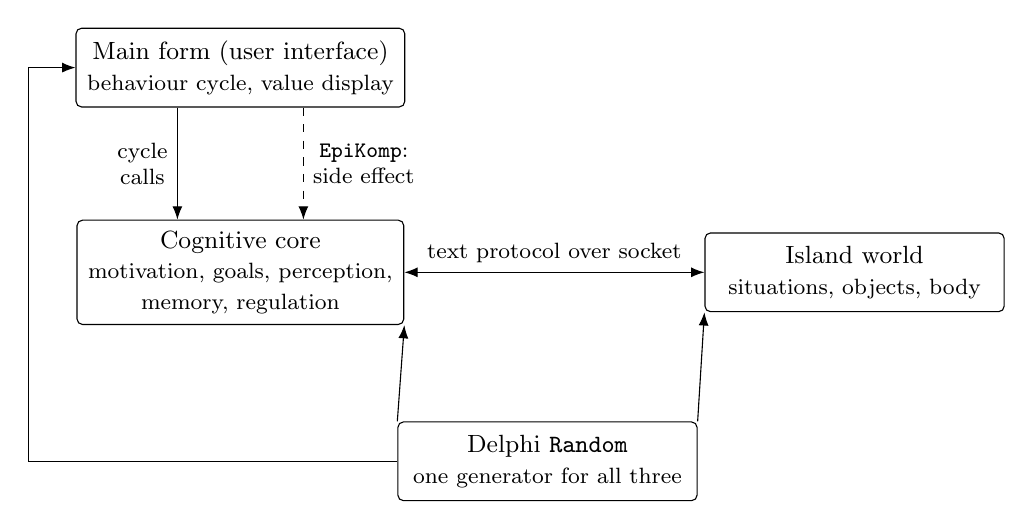
\begin{tikzpicture}[every node/.style={font=\small},
  box/.style={draw, rounded corners=2pt, align=center, minimum height=10mm, minimum width=38mm, inner sep=4pt},
  lab/.style={font=\footnotesize, align=center}]
\node[box] (form) at (0,2.6) {Main form (user interface)\\\footnotesize behaviour cycle, value display};
\node[box] (core) at (0,0) {Cognitive core\\\footnotesize motivation, goals, perception,\\\footnotesize memory, regulation};
\node[box] (world) at (7.8,0) {Island world\\\footnotesize situations, objects, body};
\node[box] (rng) at (3.9,-2.4) {Delphi \code{Random}\\\footnotesize one generator for all three};
\draw[-{Latex}] ([xshift=-8mm]form.south) -- node[left, lab]{cycle\\calls} ([xshift=-8mm]core.north);
\draw[-{Latex}, dashed] ([xshift=8mm]form.south) -- node[right, lab]{\code{EpiKomp}:\\side effect} ([xshift=8mm]core.north);
\draw[{Latex}-{Latex}] (core) -- node[above, lab]{text protocol over socket} (world);
\draw[-{Latex}] (rng.north west) -- (core.south east);
\draw[-{Latex}] (rng.north east) -- (world.south west);
\draw[-{Latex}] (rng.west) -| ([xshift=-6mm]form.west) -- (form.west);
\end{tikzpicture}
\caption{Structure of the original program. User interface, cognition and world share one random number generator, and the value display calls a function of the cognitive core that changes memory, random sequence and age (dashed). The reconstruction keeps core and world as separate objects behind a body interface, routes every draw through an explicit random source that records its call site, and keeps the display's side effect only in the reference mode.}
\label{fig:architecture}
\end{figure}

\section{Reconstruction strategy}

Agreement in every random draw requires that every source of variation be controlled. We distinguish two levels, which correspond to what \citet{axtell1996aligning} call numerical identity and distributional equivalence. At the first level, a recorded run of the original is reproduced exactly: the same random draws at the same call sites, the same protocol lines, the same actions at the same ages. At the second level, the reconstruction produces the same distribution of behaviour over many lives. This paper establishes the first level for the lives and observables listed in Table~\ref{tab:evidence}; it does not establish the second.

\paragraph{Randomness and time} As already mentioned, the user interface and the cognitive core share one random number generator. More precisely, the original draws all random numbers from Delphi's global linear congruential generator, which the user interface also uses. We reimplemented the generator bit for bit and route every draw through an explicitly passed random source that records the call site. To obtain reference sequences, we ran the original under Wine 9.0 and recorded every call of the generator with a debugger script, including the generator state before the draw and the return addresses on three levels of the call stack. The script verifies that consecutive states follow the generator's recurrence, so that a missing draw would be detected, and two recordings of seed 16 produced the same 20{,}000 draws with the same call sites. With the simulation speed set to zero, we observed no run-to-run variation of the original under Wine for a given seed; we have not compared runs under Windows, where wall-clock timers or socket timing could matter. The reconstruction has no global random state and advances in discrete cycles.

\paragraph{Arithmetic} Delphi compiles floating-point expressions for the x87 unit, which keeps intermediate results with 64-bit mantissas and rounds them to double precision when they are stored. Where such values are later printed and read back or compared, the difference to IEEE double arithmetic can change a decision \citep{monniaux2008pitfalls}. We emulate the 80-bit computation where it matters, in particular in the accumulation of the agent's age, and verified the fast path of this emulation against exact rational arithmetic.

\paragraph{Strings} The world sorts names with \code{AnsiCompareText}, whose order under Wine differs from byte order and from common locale collations. We derived a sort key that reproduces Wine's order and verified it against a comparison matrix obtained from Wine for all pairs of the 453 strings that occur in the world.

\paragraph{User interface} Where the interface changes the agent's state, the reference mode keeps the change. The most consequential case is the value display. To show the competence of each need, it calls the function that computes epistemic competence for all seven needs at the end of every cycle (form unit, lines 493 to 499), and this function draws random numbers, reinforces goal links and advances the agent's age. The machine code confirms seven calls of the same function that motive selection uses, and in the recorded draws of seed 16, 101 draws in the first 29 cycles come from these calls.

\paragraph{Tests and state} The reconstruction is guarded by characterisation tests \citep{feathers2004working}: recorded protocols and random sequences of the original serve as golden masters, and their tolerances may not be relaxed to make a test pass. The state of agent and world can be saved between two cycles and resumed in a fresh process; resumed lives are identical to uninterrupted ones. With the code of commit \code{c75ea8f} (the source and test directories are unchanged since), all 194 tests pass in a working environment that includes the original's data files (Section~\ref{sec:availability}).

\section{Validation against the original}

Table~\ref{tab:evidence} lists every life of the original that we compared with the reconstruction, with the observables compared and the first difference found. In all comparisons, wall-clock times in the protocols are replaced by a placeholder, and the separator lines of the activity protocol, which contain such times, are normalised.

\begin{table}[t]
\centering
\caption{Evidence for agreement between reconstruction (reference mode) and original under Wine. ``Protocols'': activity protocol, achievement file, interrupt-time file, activity list and end-of-life summary files. Random draws were recorded only for seed 16.}
\label{tab:evidence}
\small
\begin{tabularx}{\textwidth}{l L{0.2\textwidth} L{0.24\textwidth} Y}
\toprule
Seed & Compared & Agreement & First difference and consequence \\
\midrule
16 & Full life (739 cycles); protocols; first 75{,}000 random draws & All 109{,}140 protocol lines, 2{,}802 actions with ages, 43 process counters, summary files; draws identical in value and call site up to cycle 70 & None. The heap byte (below) was read 90 times without changing a direction \\ \addlinespace
901 & Full life (912 cycles); protocols & Actions with ages, counters and summary files identical; 90{,}697 of 90{,}698 protocol lines & One line: the heap byte turned south into a diagonal; same locomotion chosen \\ \addlinespace
1041 & Full life; protocols & All lines & None after a rounding detail in one mean of the interrupt-time file was corrected \\ \addlinespace
1061 & To cycle 204 & All lines & Reconstruction raises a nil access at cycle 204; the original stalls at the same cycle \\ \addlinespace
1035 & To cycle 380 & All actions & One line at cycle 39 (heap byte, same locomotion); nil access at cycle 380 in both \\ \addlinespace
1001 & To cycle 310 & All lines & Heap byte changes the chosen locomotion; lives diverge \\ \addlinespace
1073 & To cycle 396 & All lines & As 1001; the nil access predicted at cycle 679 is not reached by the original \\ \addlinespace
1081 & To cycle 415 & All lines & As 1001 \\ \addlinespace
1021 & To cycle 663 & All lines & As 1001 \\ \addlinespace
\bottomrule
\end{tabularx}
\end{table}

The one cause of difference that the reconstruction does not reproduce lies in the evaluation of movement directions. The original stores direction names in short strings; for the two-letter directions \code{lN} and \code{lS}, the function that evaluates a name (\code{DirArtWert}, \code{UStrukturen.Pas}, line 603) reads a third character from a local string into which only the length was copied. What it finds depends on the caller. When called from \code{ContinueDirection}, the position holds the third character of the previously examined, longer direction name; the reconstruction reproduces this stack residue. When called from \code{RememberDir}, the position holds the second byte of the address of a synapse found by the preceding call to \code{Junction}. If that byte happens to be \code{'W'} or \code{'O'}, south is read as south-west or south-east, and north correspondingly. Heap addresses depend on the allocation history of the process and cannot be derived from the program's logic. The reconstruction treats the byte as absent and reads north and south.

In the four lives in which this byte changed a choice of locomotion, original and reconstruction follow different trajectories from that cycle on. Seed-by-seed comparisons are therefore possible only for prefixes of a few hundred cycles. Beyond the divergence the two programs share their mechanism except for this byte, but whether they produce the same distribution of behaviour remains open: the reconstruction never reads a diagonal where the original sometimes does, and that difference could shift distributions. Establishing distributional equivalence would require a sufficient number of complete original lives, equivalence bounds fixed in advance and an analysis designed for equivalence; a non-significant test of difference would not suffice \citep{lakens2017equivalence}. All statements below about the original's behaviour over whole lives are therefore statements about the reconstruction in reference mode.

\section{Implementation-dependent behaviour}

Agreement at the level of individual random draws requires knowing why each draw happens. Tracing draws to their call sites exposed places at which the behaviour of the program follows from properties of its implementation and not from its published description. Table~\ref{tab:artefacts} lists them with their location in the source. The reference mode keeps these properties with one exception: of the left-over memory in direction names, it reproduces the stack residue but not the heap byte (Section~4). Each property has one switch; the modern mode switches all of them off, and for direction names this removes the stack residue. We call these properties artefacts only in the sense that they are not part of the description; we do not claim that removing them yields the only correct reading of the theory.

\begin{table}[t]
\centering
\caption{Implementation properties of the original that are not part of its description, with the switch that removes each in the reconstruction. Line numbers refer to the Delphi source of version 4.9.1.200.}
\label{tab:artefacts}
\footnotesize
\begin{tabularx}{\textwidth}{L{0.33\textwidth} Y}
\toprule
Switch and location & Property \\
\midrule
\code{background\_goals\_as\_}\newline\code{described}\newline\code{UPSIMain.Pas} 1548--1561 & The admission rule for background goals reduces to $P = \textit{strength} \times \textit{threshold}$, which grows with the strength of the current motive; the book states $P = \textit{need} - \textit{strength} \times \textit{threshold}$ \\ \addlinespace
\code{no\_display\_side\_effects}\newline\code{UFPsi.pas} 493--499 & The value display computes epistemic competence for all needs each cycle, drawing random numbers, reinforcing goal links and advancing age \\ \addlinespace
\code{goal\_in\_current\_situation}\newline\code{PlanenUndTun} & A parameter named \code{situation} shadows the global current situation, so after a plan that moves the agent the goal is sought in the situation it left \\ \addlinespace
\code{clean\_direction\_names}\newline\code{UStrukturen.Pas} 603 & Direction names \code{lN} and \code{lS} are evaluated with a third character from left-over stack or heap memory \\ \addlinespace
\code{aversion\_check\_in\_aversions}\newline\code{Consum} (\code{UAction.pas}) & When an object proves harmful, the check for an existing aversion looks in the goal links; known aversions are never reinforced \\ \addlinespace
\code{guard\_nil\_dereferences}\newline\code{ActivateAuto}, \code{Confirmation} & Pointers are followed without a nil check; a protocol chain that ends early raises an access violation \\ \addlinespace
\code{real\_umlaut\_bitmaps}\newline(Wine) & Bitmaps whose file names contain an umlaut are not found under Wine and are drawn as text; an effect of the environment, not of the program \\ \addlinespace
\bottomrule
\end{tabularx}
\end{table}

The admission rule for background goals is the property with the clearest relation to the theory. For each goal of a need $i$ other than the current motive, the original computes $r = a_i \cdot w_{\text{link}} \cdot g_i$, the activity of the need times the weight of the goal link times the weight of the need, then $s = r - m \cdot \theta$, with $m$ the activity of the current motive's need and $\theta$ the selection threshold, and admits the goal if a uniform random number is smaller than $r - s$ (\code{UPSIMain.Pas}, lines 1548 to 1561). Since $r - s = m \cdot \theta$, the probability of admitting a background goal is independent of the need it serves and grows with the strength of the current motive. (As an example, with the nucleotide need as current motive at an activity of about 0.67 and the threshold near its observed mean of 0.065, this probability is about 0.04.) The book states the rule as $\textit{random} < \textit{BedIn}_i - \textit{MotivStaerke} \times \textit{SelectSchwelle}$ and illustrates it with two worked examples in which the probability falls as the current motive grows stronger \citep[p.~99]{doerner2002mechanik}; under this rule the probability is $\max(0, s)$, depends on the need, and can be zero. The code thus implements the opposite dependence on the current motive from the one described, at a place that the book presents as the mechanism of the breadth of attention. The switch replaces $r - s$ by $s$, which is the book's rule with the program's definition of the need term.

The shadowed situation in planning and the side effects of the display were found because draws occurred at unexpected call sites: in the random recording of seed 16, the display accounts for 101 draws in the first 29 cycles, and the shadowed parameter showed up as a search for a goal object in a situation the agent had already left at cycle 65. The remaining properties are of a different kind. The direction residue has already been discussed in Section~4. The unguarded pointers matter because of their consequence: in the original, an access violation aborts the cycle, and because a flag that would restart the simulation is not reset, the life then stalls without ending.

\paragraph{Lives that stall} Of 100 reconstructed reference lives (seeds 1001 to 1100), 97 ran to the configured age and 3 stalled on a nil access: seeds 1035 and 1061 in \code{ActivateAuto} at cycles 380 and 204, and seed 1073 in \code{Confirmation} at cycle 679. A stall is a failure of the software, distinct from the agent's death. For seeds 1035 and 1061 the original stalled at the same cycle; for seed 1073 the original had diverged earlier and did not reach the predicted location. The rate of 3 in 100 is therefore a property of the reconstruction in reference mode with this configuration, of which two cases are confirmed in the original. In the modern mode all 100 lives completed; the guard intervened once each in seeds 1025 and 1030.

\paragraph{Effect of the properties on behaviour} We compared the modern mode with the reference mode on six measures: deaths per 1{,}000 cycles (P1), nucleotides per 100 cycles (P2), locations discovered (P3), success rate of manipulations (P4), share of cycles with trial and error (P5) and the mean strength of the damage need over cycles (P6). The analysis is restricted to the 97 seeds in which the reference life completed, so it estimates the effect conditional on a complete reference life. Differences were paired by seed and tested with a sign-flip permutation test (10{,}000 permutations) with bootstrap percentile intervals (10{,}000 resamples), both with fixed seeds; the Holm correction was applied to the six $p$ values, not to the intervals, which are pointwise. Pairing by seed compares lives from identical initial states, but because the switches change the number of random draws, later decisions use different random numbers; the comparison therefore measures the joint effect on whole lives and does not isolate local mechanisms.

{\footnotesize\setlength{\tabcolsep}{1.8pt}\begin{table}[t]
\centering
\caption{Modern against reference mode over the 97 seeds of 1001 to 1100 in which the reference life completed. Means per mode; difference modern minus reference, paired by seed, with pointwise 95\% bootstrap interval; p from a sign-flip permutation test, Holm-adjusted across the six measures.}
\label{tab:T3}
\begin{tabular}{lrrrlr}
\toprule
Measure & Reference & Modern & Difference & 95\% CI & p (Holm) \\
\midrule
P1 Deaths per 1,000 cycles & 11.954 & 9.345 & -2.609 & [-3.065, -2.152] & $<$ 0.001 \\
P2 Nucleotides per 100 cycles & 13.861 & 13.701 & -0.161 & [-0.540, 0.213] & 0.405 \\
P3 Locations discovered & 96.567 & 98.186 & 1.619 & [0.639, 2.608] & 0.005 \\
P4 Manipulation success (share) & 0.378 & 0.397 & 0.020 & [0.013, 0.027] & $<$ 0.001 \\
P5 Trial-and-error cycles (share) & 0.855 & 0.788 & -0.068 & [-0.076, -0.061] & $<$ 0.001 \\
P6 Damage need (\%) & 75.544 & 67.042 & -8.502 & [-9.536, -7.446] & $<$ 0.001 \\
\bottomrule
\end{tabular}
\end{table}
}

Table~\ref{tab:T3} shows that without the implementation properties the agent died less often than it did with them (9.35 instead of 11.95 deaths per 1{,}000 cycles), its damage need was lower (67.0 instead of 75.5\,\%), its manipulations succeeded more often, it discovered slightly more locations and relied less on trial and error; its rate of collecting nucleotides did not differ reliably. Because rates per cycle depend on the number of cycles, and because the switches change how much model time a cycle takes, we checked the two largest effects against other measures of exposure (all paired over the same 97 seeds, computed after the original analysis). Lives had similar numbers of cycles in both modes ($925.5 \pm 72.0$ and $929.4 \pm 68.7$, mean $\pm$ SD). Deaths per 1{,}000 actions fell by 0.78 (95\,\% CI $-0.92$ to $-0.65$), deaths per million units of model time by 0.47 ($-0.58$ to $-0.37$), and over the first $n$ cycles of each pair, with $n$ the length of the shorter life, deaths per 1{,}000 cycles by 2.51 ($-2.95$ to $-2.07$). The damage need weighted by model time instead of cycles fell by 9.1 percentage points ($-10.7$ to $-7.5$). Deaths are recurring events within a life, after which the agent restarts; they are counted per life and are not independent observations of survival.

A screening of the individual switches over 20 seeds, which preceded this comparison, found the largest single effects for the background-goal rule (deaths $-2.6$ per 1{,}000 cycles) and for the shadowed situation in planning (nucleotides $+1.3$ per 100 cycles), and no reliable effects for the display, the aversion check and the bitmaps. These single-switch results are exploratory; they were not confirmed with 100 seeds, and because the switches may interact, they do not determine shares of the joint effect.

\paragraph{Provenance of the modern-mode runs} The first 20 modern-mode lives were run before the nil guard existed and therefore list six switches in their metadata; the other 80 list seven. The guard acts only when a nil access occurs, and none of the first 20 lives raised one, so they are identical to runs with the guard switched on. A per-seed manifest lists the switches, the guard interventions and a hash of every run file.

\paragraph{Dominance of one motive} On this island one motive almost always holds control. In the 97 complete reference lives, nucleotides were the current motive in 99.89\,\% of the 89{,}775 motive decisions recorded in the protocols (pooled over lives); the mean share per life was 99.89\,\% (SD 0.30 percentage points, lowest life 97.6\,\%), and 65 lives never switched motive, while in the others thirst or hunger took over for brief episodes. In the modern mode 99 of 100 lives never switched. The motive strengths show why. In a complete modern life (seed 1001) the nucleotide motive had a mean strength of 0.47 and a maximum of 0.49, the strongest competing motive never exceeded 0.43, and the selection threshold stayed between 0.034 and 0.090 over 20 lives. The nucleotide need rises and falls fast (rate 0.1 in both directions) and is weighted 0.7, while energy and water change by orders of magnitude more slowly (Table~\ref{tab:params}). We attribute the dominance to this world and parameter set and not to the theory. Thus, studies of motive selection on this island exercise the selection rule only weakly.

\section{Discussion}

The reconstruction agrees with the original in every compared observable of a complete reference life and of a second complete life except for one protocol line, and in the prefixes of seven further lives up to the first change caused by a heap byte that cannot be reproduced from the program's logic. Two points stand out against the background of the replication literature. First, the most consequential difference between description and program was found by asking why a random draw happened at a particular call site; a comparison of outputs had not revealed it. An alignment at the level of distributions, as is usual for simulation models \citep{axtell1996aligning,wilensky2007making}, would have tested whether the reconstruction behaves like the original, and it would not have revealed that both implement a background-goal rule that inverts the book's. Second, properties of the implementation changed the agent's survival by amounts comparable to effects one would study experimentally. \citet{edmonds2003replication} reported a similar experience for a model of cooperation, where an undescribed rule for resolving ties changed the results.

These findings concern any work that uses the program as a model of the theory, including earlier comparisons with human behaviour \citep{doerner2004emotions}. We do not know which version of the software those studies used, and we therefore make no claim about the properties of the agents in them. The general consequence is that a comparison between a program and human data validates the program as it ran, and that the theory as written and the theory as run can differ in ways that matter for behaviour.

The dominance of the nucleotide motive is of the same kind. Anyone who uses the island to study motive selection, emotional modulation or the flexibility of behaviour has to take into account that, with these parameters, the motive hardly ever changes.

We have to take into account that our results might apply only to the configuration we studied, and the work has limitations beyond the open question of distributional equivalence. The comparisons were run under Wine on Linux and not under Windows. They cover the island program with one parameter file; the later population model of the same group is not reconstructed. The individual switches were screened over 20 seeds and not confirmed. The comparison of the modes is conditional on complete reference lives and does not count the reference mode's stalls as outcomes. Finally, the effects of the modern mode are effects of removing all listed properties together, measured in one world.

In conclusion, we can say that the island program can now be run, inspected and varied outside its original environment, and that the reconstruction reproduces the original wherever the original's behaviour follows from its own logic. Further work will be needed to establish whether the two programs agree in distribution, and to examine which of the documented properties were present in the versions used in earlier studies with the agent.

\section{Availability and reproducibility}
\label{sec:availability}

The reconstruction, its tests, the analysis scripts, the data of all runs reported here and a per-seed manifest are available in a public repository (\url{https://github.com/alec85/doerner-psi-island}; code under the MIT License, data under CC BY 4.0), with an archived version for this paper \todo{DOI}. The repository also contains the protocols of all runs of the original under Wine that this paper compares, unchanged as the program wrote them, together with their converted form. The original Delphi source code, the executable and its data files are not part of that repository.

The reconstruction needs four categories of files from the original distribution: three for every run of the Python program (the parameter file, five world files and 267 bitmap files) and one, the executable, only for runs of the original under Wine and for the tests that read it. The repository lists all 274 files with their ordinary SHA-256 sums in a form that \code{sha256sum -c} checks, so that a reader with a copy of the original can verify that it is the same material; the script that writes this list stops with an error if a required file or directory is missing. Without these files no new life can be run, and 63 of the 194 tests fail or cannot be set up.

Everything reported in this paper can nevertheless be recomputed from archived data. The repository contains the run traces of all 200 baseline lives and, for quantities that the traces do not hold (numbers of actions, motive reports, guard interventions, the parameter values), a table extracted once from the complete runs, with the SHA-256 sums of the files each value was taken from. A single script verifies the archives, extracts them, recomputes all analyses and the tables of the paper and compares every value with the committed results. We ran it in a fresh copy of the repository without the original files, at the commit of the analysis code (\code{ecc08a0}); every value was reproduced exactly. Figures are regenerated by the same tools but not compared byte for byte.

The baseline runs were produced on 10 and 11 November 2026 with versions of the reconstruction whose commits were not stored in the run files; the runs are identified by the hashes in the manifest. The code of the reconstruction described here is commit \code{c75ea8f}. All runs and analyses used Python 3.13 with NumPy 2.5; the original ran under Wine 9.0 on Ubuntu 24.04. On one core of an Intel Xeon processor at 2.1\,GHz (virtual machine with two cores and 7\,GB of memory), a reference-mode life of 945 cycles took 132\,s.

\paragraph{Use of AI tools} The reconstruction, its tests and the analysis scripts were written by an AI coding agent, Claude Code with Anthropic's model Claude Opus~5.5, which worked in the project repository under the author's direction. The author set the research questions and the analysis plans and took the decisions that the repository records as architecture decision records; the agent implemented them, ran the experiments and reported the results. Every number in this paper comes from executed code and can be recomputed with the script described above. The characterisation tests against the original guard the code, and their tolerances were not relaxed at any point. The repository keeps the complete history of these steps.

\section*{Declaration of generative AI and AI-assisted technologies in the writing process}

During the preparation of this work the author used Claude Code (Anthropic, model Claude Opus~5.5) in order to draft and revise the text, tables and figures and to check every statement against the repository, and OpenAI Codex (model GPT 6.1 Sol) in order to obtain two rounds of critical review of the manuscript. After using these tools, the author reviewed and edited the content as needed and takes full responsibility for the content of the publication.

\section*{Declaration of competing interest}

The author declares that he has no known competing financial interests or personal relationships that could have appeared to influence the work reported in this paper.

\section*{Funding}

This research did not receive any specific grant from funding agencies in the public, commercial, or not-for-profit sectors.

\section*{CRediT authorship contribution statement}

\textbf{Alec Sproten:} Conceptualization, Methodology, Resources, Validation, Project administration, Writing -- review \& editing.

\section*{Data availability}

Code, run data, the protocols of the compared runs of the original and the analysis scripts are available as described in Section~\ref{sec:availability}. The original Delphi program and its data files cannot be shared by the author.

\bibliographystyle{elsarticle-harv}
\bibliography{referenzen}

\end{document}
